\newpage

\begin{lstlisting}[language=JuliaLocal, style=julia]
using PlutoUI
\end{lstlisting}

\begin{lstlisting}[language=JuliaLocal, style=julia]
begin
	using Plots
	y(x) = sin(x)
	plot(y,
		color=:blue)
end
\end{lstlisting}

\begin{figure}[H]
	\centering
	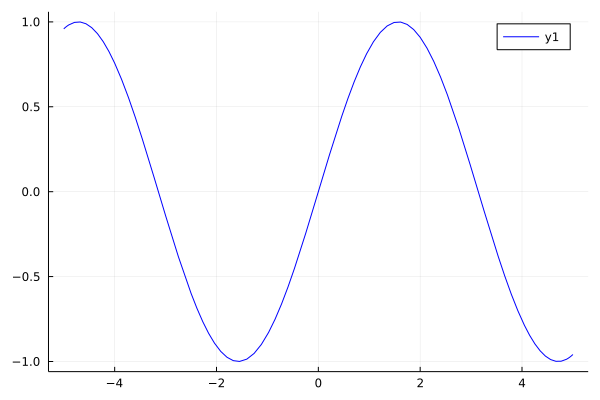
\includegraphics[width=0.8\textwidth]{./figures/examplepluto_figure1.png}
	\label{fig:examplepluto_figure1.png}

\end{figure}

\begin{lstlisting}[language=JuliaLocal, style=julia]
A = [10,10,10]
\end{lstlisting}

\begin{verbatim}
3-element Vector{Int64}:
 10
 10
 10
\end{verbatim}

\begin{lstlisting}[language=JuliaLocal, style=julia]
x = rand(10);
\end{lstlisting}

\begin{lstlisting}[language=JuliaLocal, style=julia]
x .+ 1
\end{lstlisting}

\begin{verbatim}
10-element Vector{Float64}:
 1.5462258585184834
 1.422347434043814
 1.4436678563913414
 1.1933180031129502
 1.9066232927293663
 1.0065197398699526
 1.2180164100462618
 1.3150502497411913
 1.907827947811504
 1.5508272577240927
\end{verbatim}

\begin{lstlisting}[language=JuliaLocal, style=julia]
set_theme!(theme_ggplot2())
\end{lstlisting}

\begin{lstlisting}[language=JuliaLocal, style=julia]
Makie.plot(x)
\end{lstlisting}

\begin{figure}[H]
	\centering
	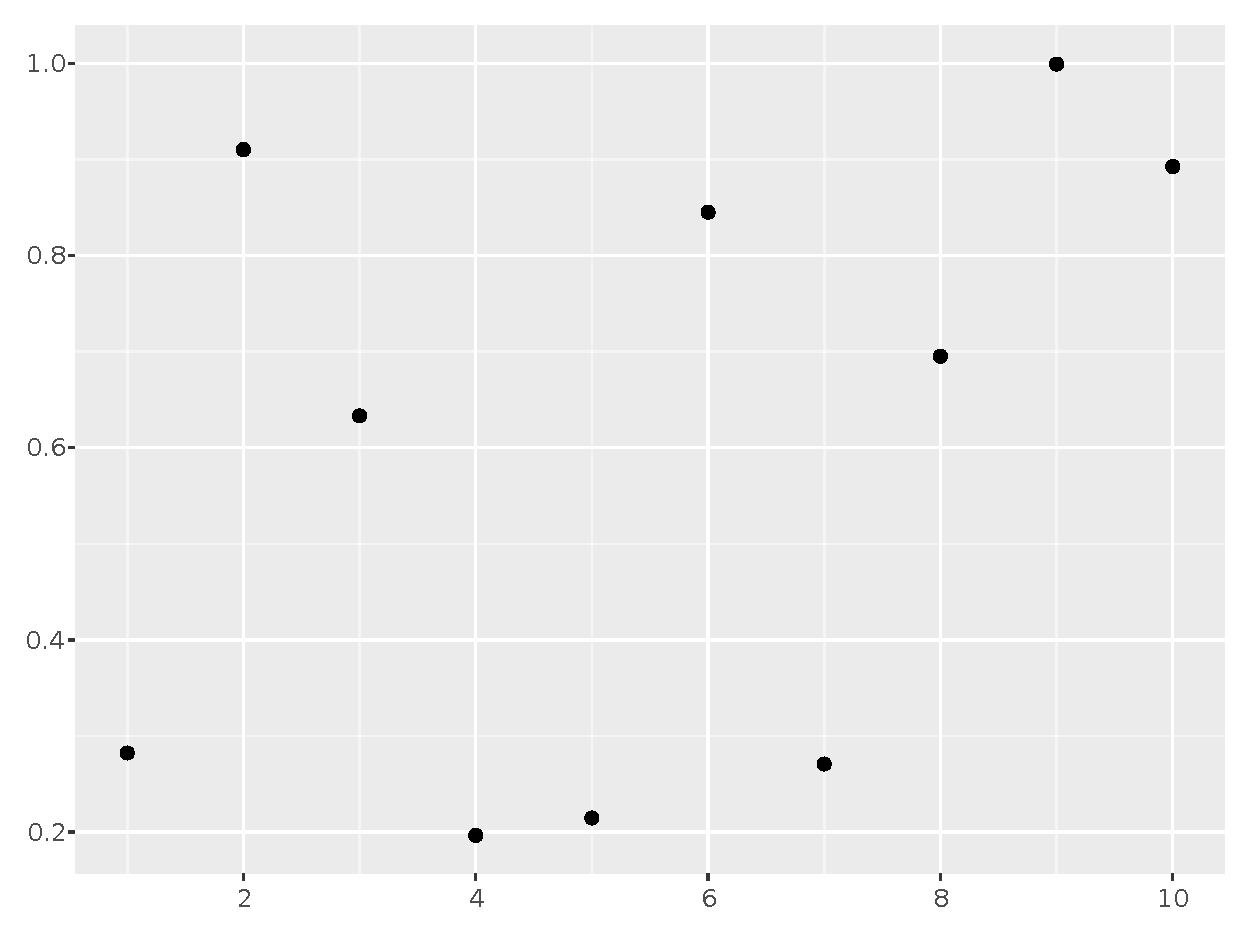
\includegraphics[width=0.8\textwidth]{./figures/examplepluto_figure2.pdf}
	\label{fig:examplepluto_figure2.pdf}

\end{figure}

\begin{lstlisting}[language=JuliaLocal, style=julia]
PlutoUI.LocalResource(figurepath)
\end{lstlisting}

\begin{figure}[H]
	\centering
	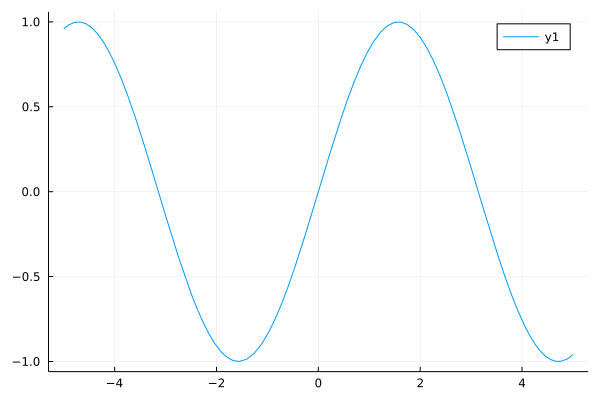
\includegraphics[width=0.8\textwidth]{/home/davibarreira/MEGA/EMAp/PlutoLatexConverter.jl/example/plotexample.png}
	\label{fig:/home/davibarreira/MEGA/EMAp/PlutoLatexConverter.jl/example/plotexample.png}

\end{figure}
